\chapter{Resultados e Discussão}

Esta seção apresenta os resultados obtidos a partir dos procedimentos de validação descritos no Capítulo 4 e discute seu significado no contexto da arquitetura desenvolvida.

Os resultados são organizados de acordo com os principais módulos avaliados: simulações elétricas do circuito de acionamento, implementação computacional, comunicação UDP, validação física do canal vibrotátil, ensaio com estímulo mecânico controlado, caracterização acústica do atuador, alimentação embarcada, feedback visual e operação integrada do sistema.

A análise concentra-se nos aspectos técnicos e funcionais do protótipo, considerando a aquisição dos eventos MIDI, o processamento do parâmetro \textit{velocity}, o mapeamento para os comandos PWM, a transmissão das mensagens ao ESP32 e a geração simultânea dos feedbacks vibrotátil e visual.

Como o trabalho não contempla ensaios clínicos nem estudos formais de percepção com participantes, as discussões apresentadas nesta seção permanecem restritas aos resultados técnicos, computacionais, elétricos e funcionais observados durante os experimentos.


\section{Resultados das Simulações Elétricas}
\markright{Resultados e Discussão}
\label{sec:resultados_simulacoes_eletricas}

As simulações descritas na Seção~\ref{sec:simulacao_circuito} foram utilizadas para avaliar qualitativamente o comportamento do estágio eletrônico de acionamento antes da integração física completa do protótipo.

A análise considerou dois aspectos principais: a influência do diodo de \textit{flyback} durante o chaveamento da carga indutiva e o comportamento do circuito diante de diferentes valores de \textit{duty cycle} do sinal PWM.

Os resultados apresentados nesta seção devem ser interpretados como uma análise do comportamento elétrico do modelo equivalente utilizado no LTspice, não correspondendo a uma caracterização completa do comportamento eletromecânico do motor Vibracall 1027.


\subsection{Proteção por Diodo de \textit{Flyback}}
\markright{Resultados e Discussão}
\label{sec:resultado_flyback}

A Figura~\ref{fig:simulacao_com_flyback} apresenta a resposta transitória do circuito utilizando o diodo de \textit{flyback} em paralelo com a carga indutiva equivalente.

\begin{figure}[!htbp]
\centering
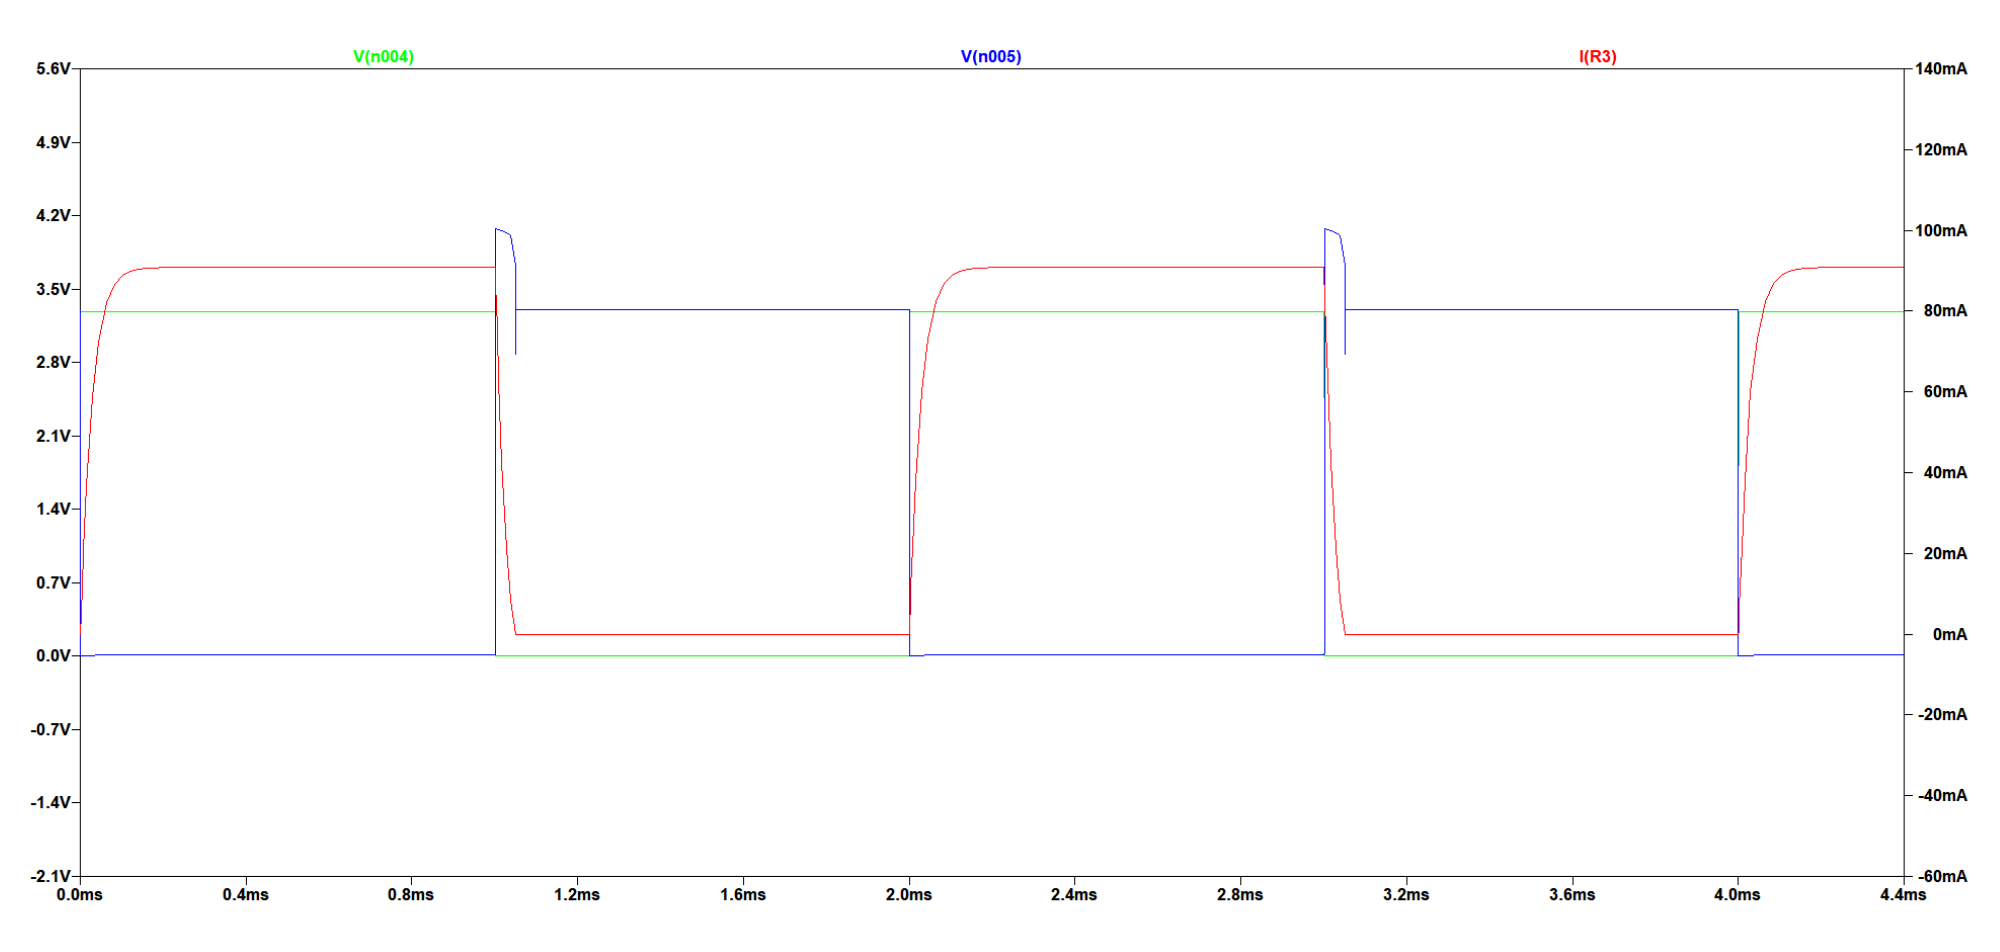
\includegraphics[
width=0.95\linewidth,
keepaspectratio
]{Metodologia/simulacao_com_flyback.png}
\caption{Resposta transitória do circuito utilizando diodo de \textit{flyback}}
\label{fig:simulacao_com_flyback}
\legend{Fonte: Elaboração própria (2026).}
\end{figure}

Na condição simulada com o diodo, os transitórios de tensão associados à interrupção da corrente na carga indutiva foram limitados pela existência de um caminho de recirculação de corrente.

A Figura~\ref{fig:simulacao_sem_flyback} apresenta o comportamento do mesmo circuito na ausência do diodo de proteção.

\begin{figure}[!htbp]
\centering
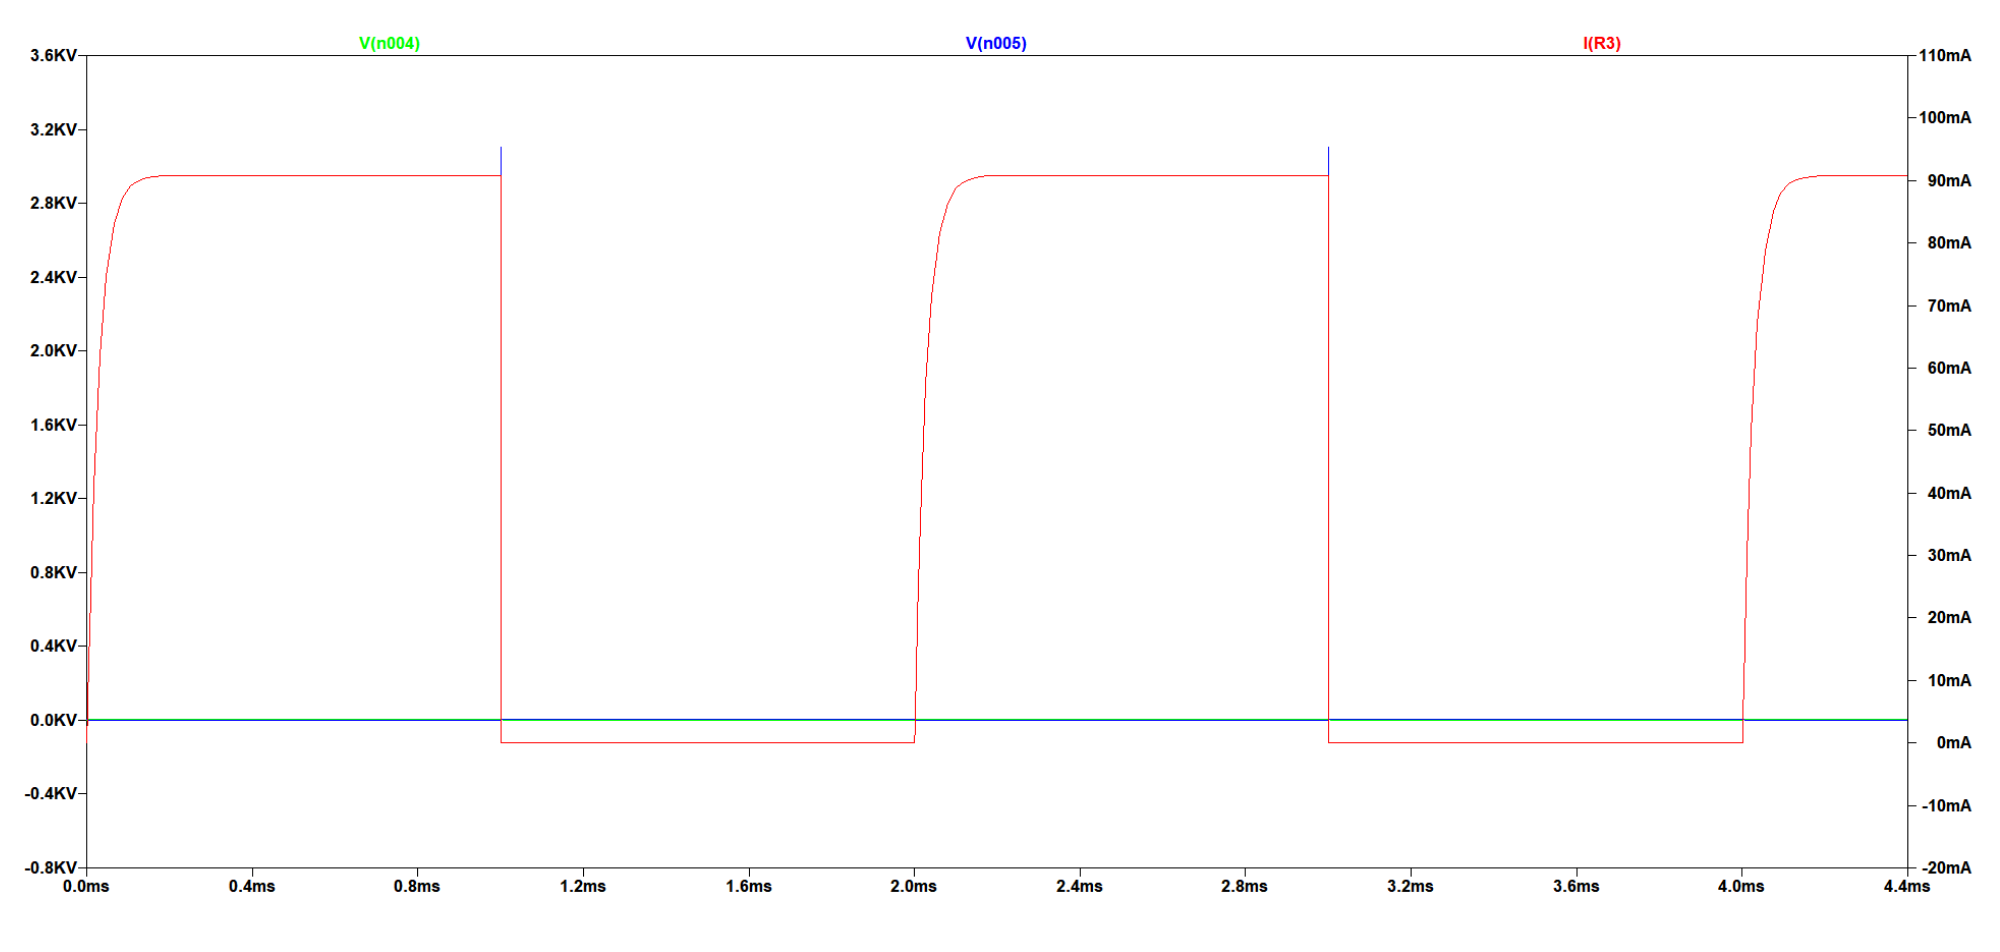
\includegraphics[
width=0.95\linewidth,
keepaspectratio
]{Metodologia/simulacao_sem_flyback.png}
\caption{Resposta transitória do circuito sem diodo de \textit{flyback}}
\label{fig:simulacao_sem_flyback}
\legend{Fonte: Elaboração própria (2026).}
\end{figure}

Nessa condição, a simulação apresentou transitórios de tensão mais pronunciados durante o desligamento da carga.

A comparação entre os dois cenários evidencia qualitativamente a função do diodo de \textit{flyback} no estágio de acionamento, justificando sua utilização em paralelo com o motor vibrotátil do protótipo.

Deve-se considerar, entretanto, que os valores absolutos obtidos dependem das simplificações adotadas no modelo elétrico e não devem ser interpretados como reprodução exata do comportamento físico do motor Vibracall 1027.




\subsection{Comportamento do Controle PWM}
\markright{Resultados e Discussão}
\label{sec:resultado_pwm_simulacao}

As simulações realizadas com diferentes valores de \textit{duty cycle} permitiram comparar o comportamento elétrico do modelo equivalente do atuador vibrotátil para diferentes níveis de comando PWM.

A Figura~\ref{fig:pwm20_resultado} apresenta a resposta obtida para um \textit{duty cycle} de 20\%.

\begin{figure}[!htbp]
    \centering
    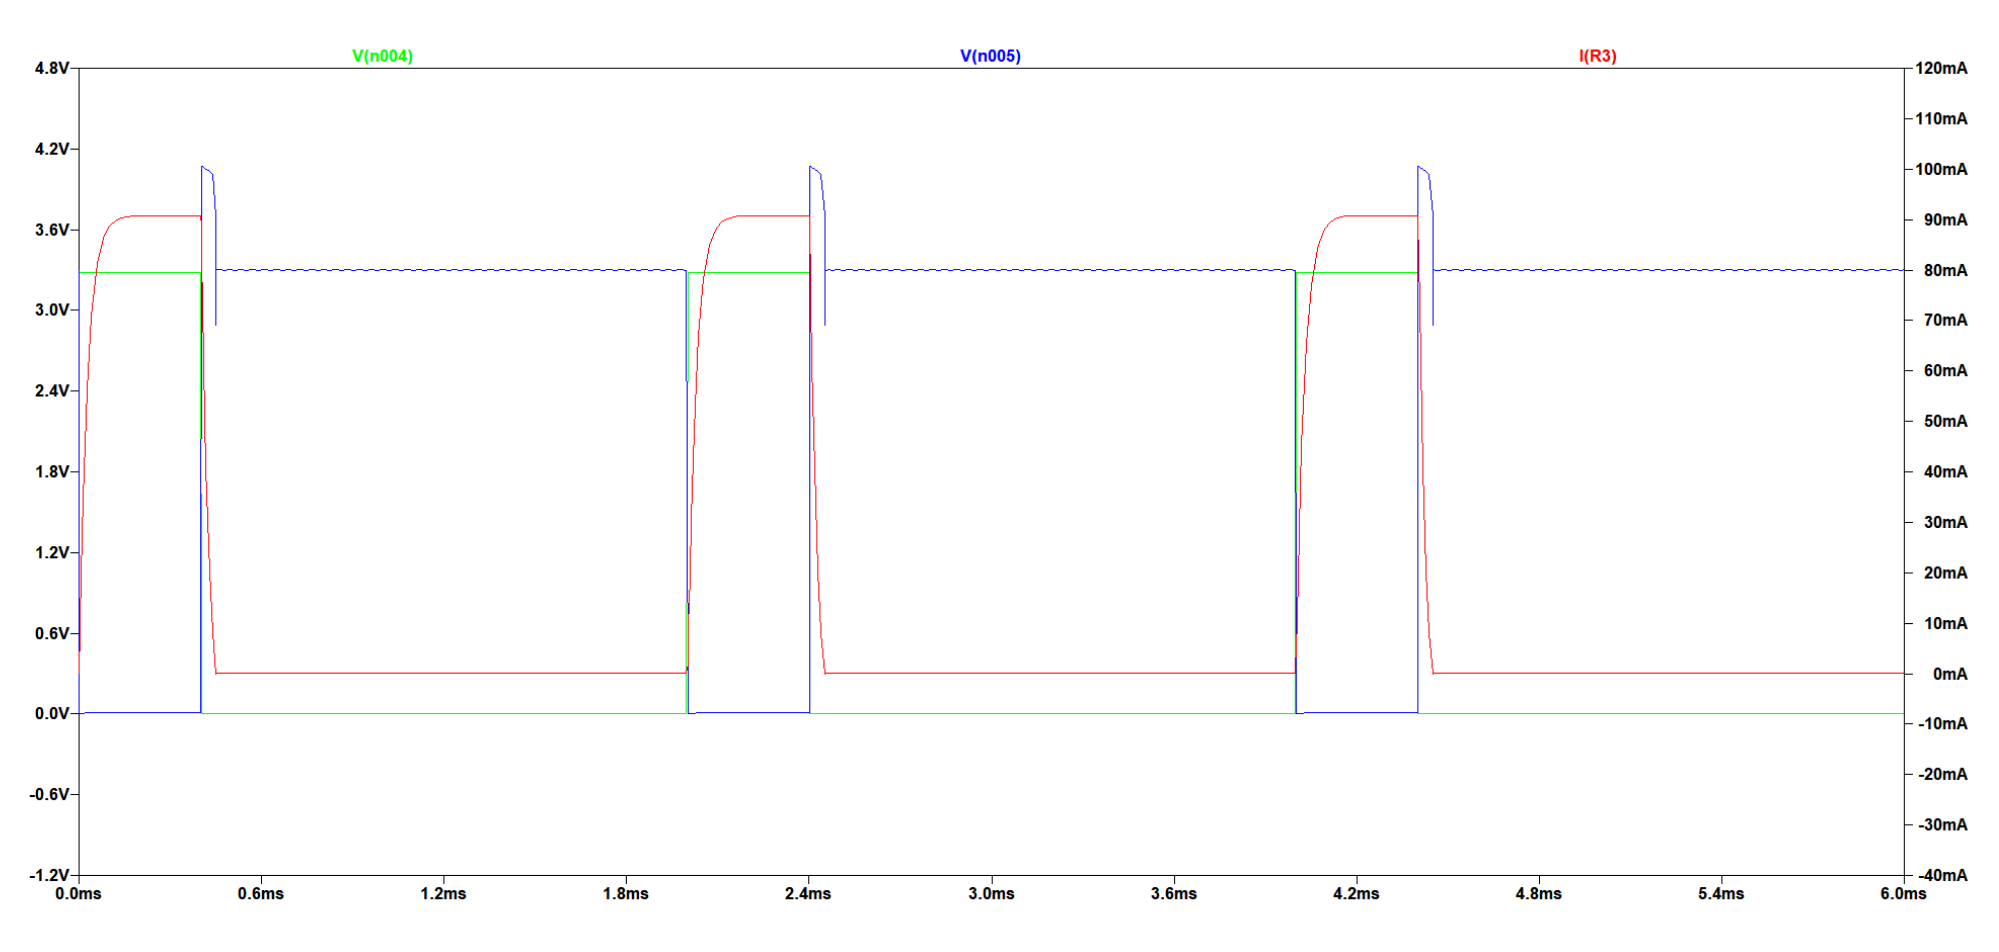
\includegraphics[
        width=0.95\linewidth,
        keepaspectratio
    ]{Metodologia/simulacao_pwm_20.png}
    \caption{Resposta simulada do circuito para \textit{duty cycle} de 20\%}
    \label{fig:pwm20_resultado}
\legend{Fonte: Elaboração própria (2026).}
\end{figure}

Nessa condição, o modelo apresentou o menor valor médio de corrente na carga entre os três cenários analisados.

A Figura~\ref{fig:pwm50_resultado} apresenta a resposta obtida para um \textit{duty cycle} de 50\%.

\begin{figure}[!htbp]
    \centering
    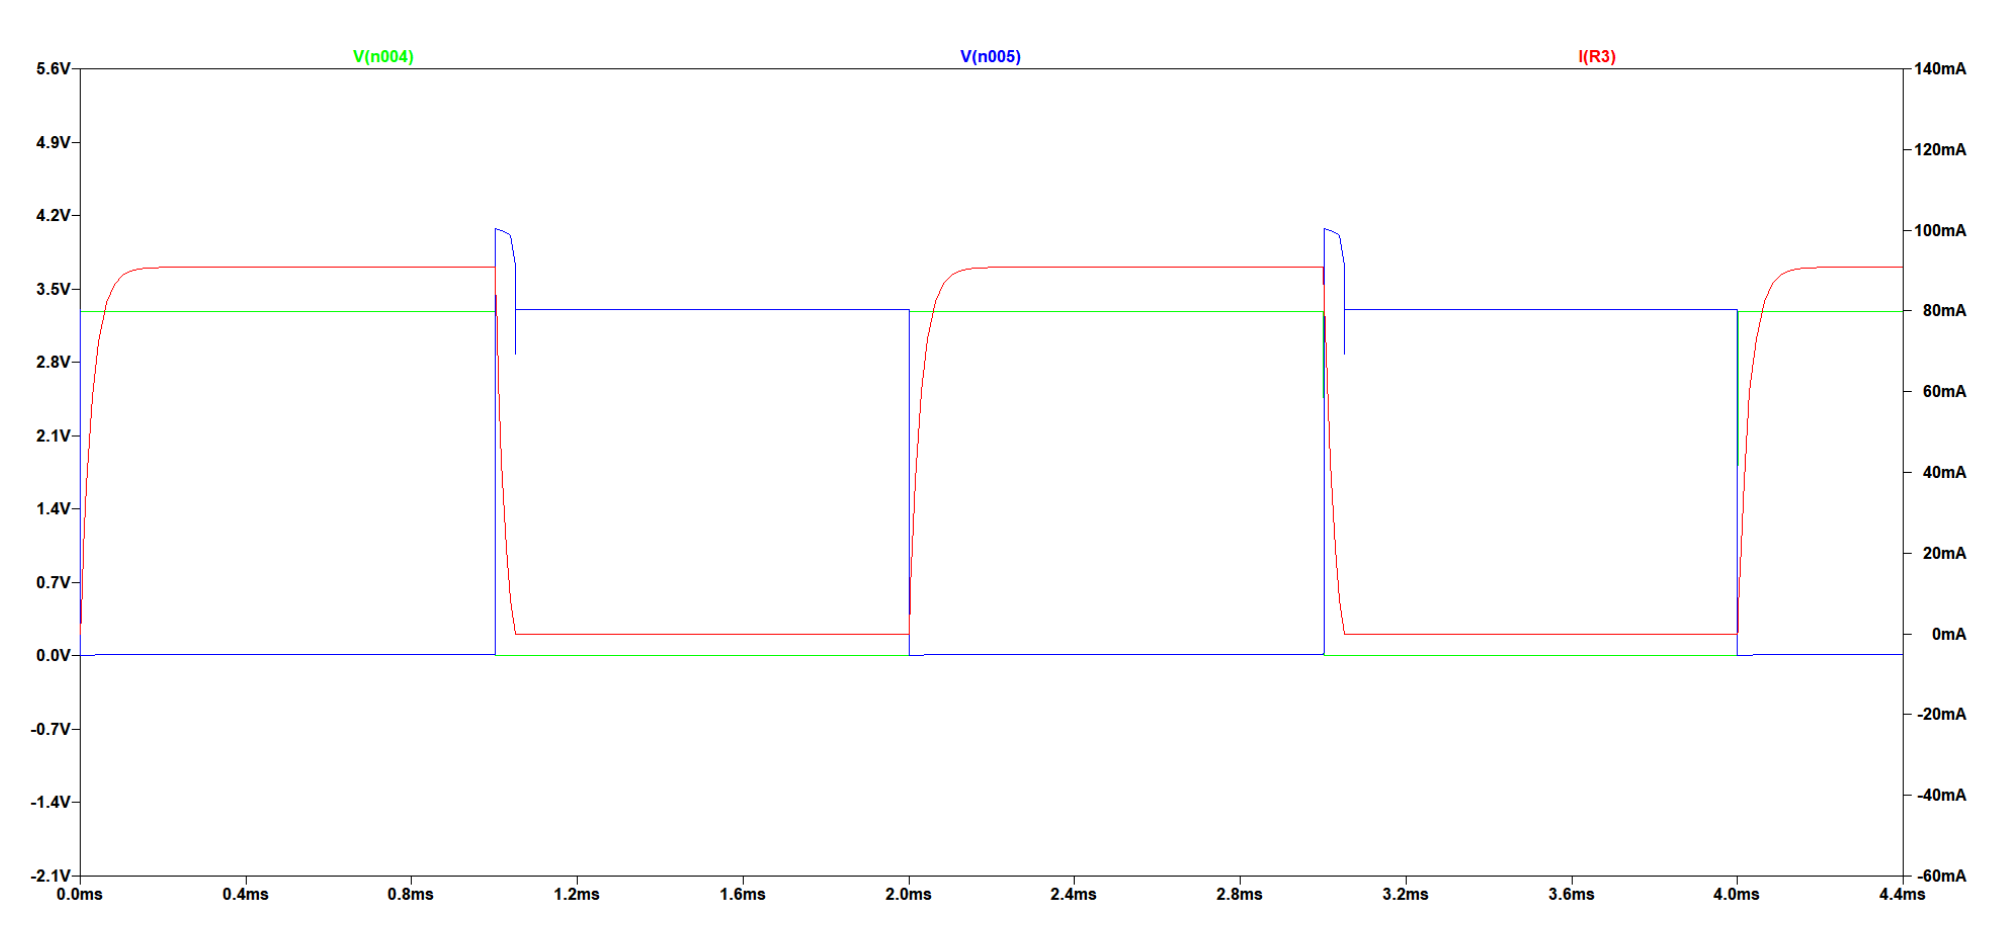
\includegraphics[
        width=0.95\linewidth,
        keepaspectratio
    ]{Metodologia/simulacao_pwm_50.png}
    \caption{Resposta simulada do circuito para \textit{duty cycle} de 50\%}
    \label{fig:pwm50_resultado}
\legend{Fonte: Elaboração própria (2026).}
\end{figure}

Para a condição intermediária, observou-se aumento do valor médio de corrente na carga em relação à condição de 20\%.

A Figura~\ref{fig:pwm80_resultado} apresenta a resposta obtida para um \textit{duty cycle} de 80\%.

\begin{figure}[!htbp]
    \centering
    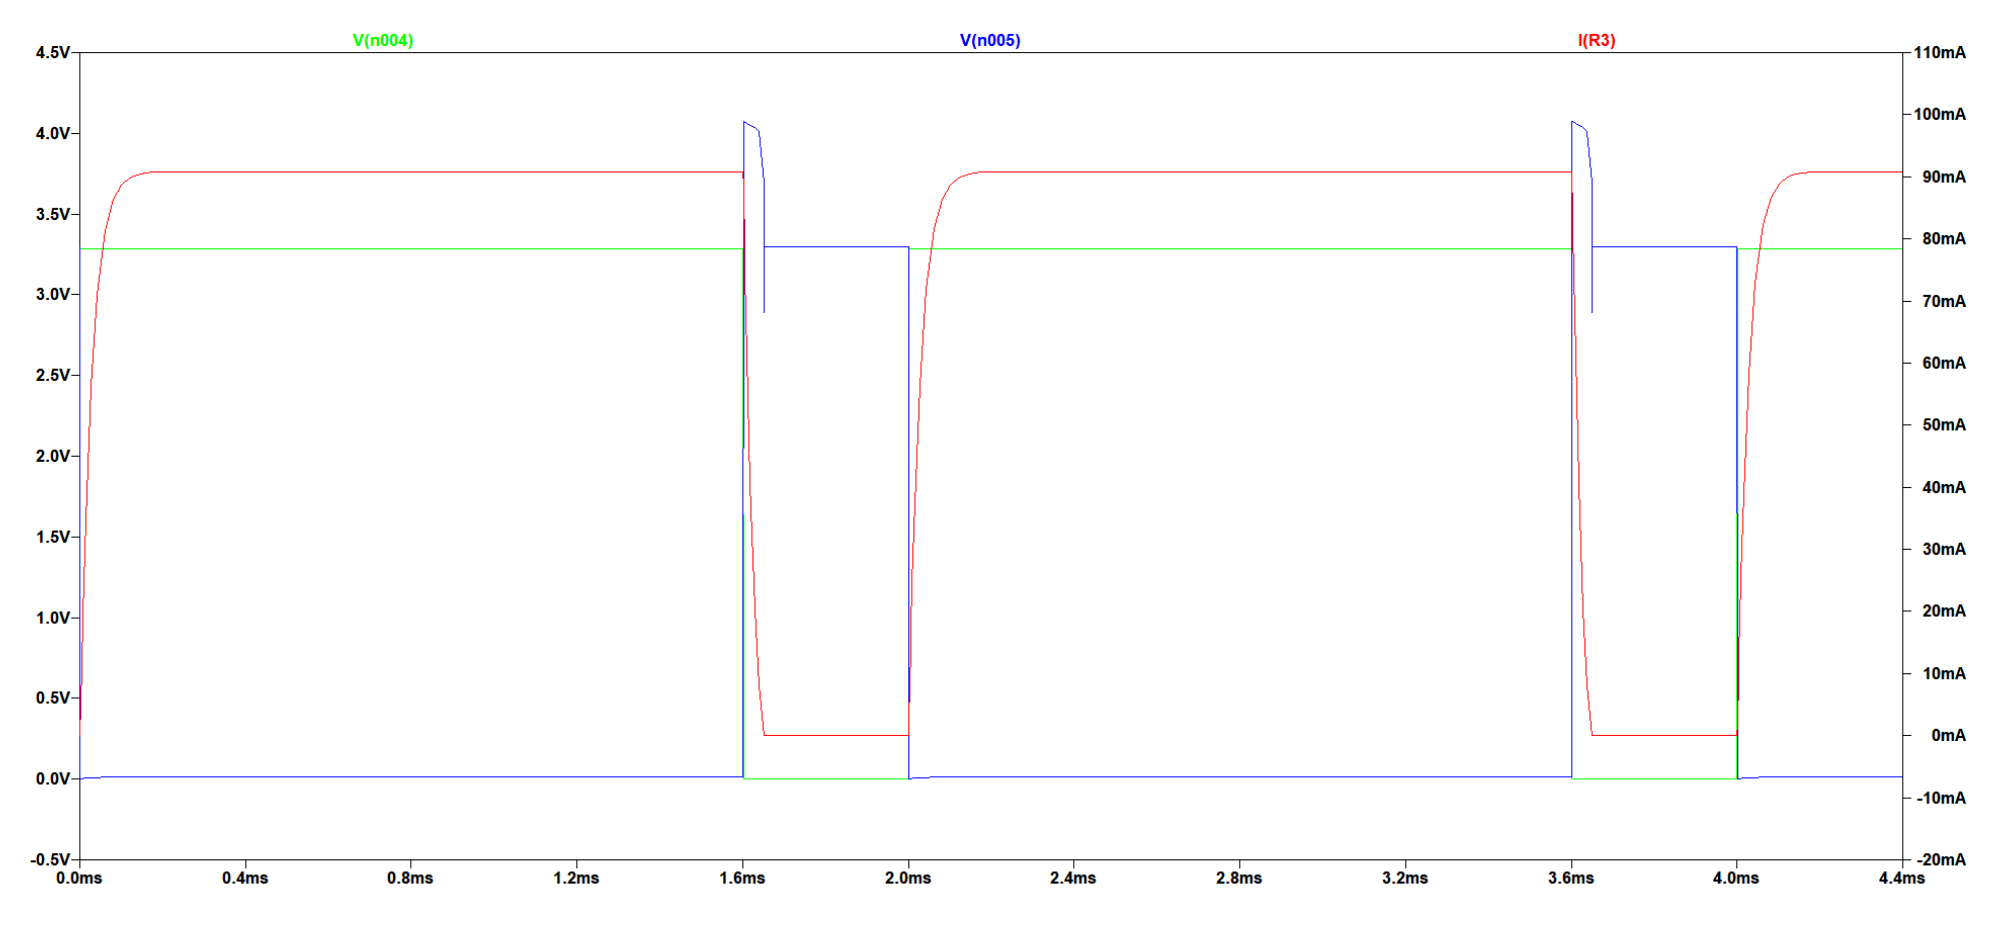
\includegraphics[
        width=0.95\linewidth,
        keepaspectratio
    ]{Metodologia/simulacao_pwm_80.png}
    \caption{Resposta simulada do circuito para \textit{duty cycle} de 80\%}
    \label{fig:pwm80_resultado}
\legend{Fonte: Elaboração própria (2026).}
\end{figure}

A condição de 80\% apresentou o maior valor médio de corrente entre os três cenários analisados.

A comparação entre as simulações de 20\%, 50\% e 80\% mostrou que o aumento do \textit{duty cycle} resulta em aumento da energia média fornecida à carga equivalente.

Esse comportamento é compatível com a estratégia adotada no protótipo, na qual o valor PWM é utilizado como variável de controle do canal vibrotátil.

Os resultados fornecem suporte elétrico para a utilização de diferentes valores PWM como níveis distintos de comando do motor Vibracall 1027.

Entretanto, as simulações não permitem estabelecer, por si só, uma relação quantitativa entre o valor PWM aplicado, a amplitude mecânica da vibração produzida pelo motor e a intensidade percebida pelo usuário.

Embora o mesmo valor PWM seja posteriormente utilizado como referência para o canal visual, as simulações apresentadas nesta seção representam exclusivamente o estágio eletrônico associado ao atuador vibrotátil e não caracterizam o comportamento luminoso do LED.


\section{Validação da Implementação Computacional}
\markright{Resultados e Discussão}
\label{sec:resultados_implementacao_computacional}


A implementação computacional foi avaliada inicialmente de forma independente do estágio físico de acionamento, conforme o procedimento descrito no Capítulo 4.

Essa etapa permitiu verificar a aquisição dos eventos MIDI, a extração do parâmetro \textit{velocity}, o cálculo dos valores PWM e a geração dos comandos antes da integração completa com o ESP32 e com as modalidades físicas de feedback.

Também foi verificado o funcionamento da interface gráfica desenvolvida para acompanhamento da interação, permitindo observar durante os ensaios o pad acionado, o valor de \textit{velocity} e o valor PWM calculado.

\subsection{Aquisição e Processamento dos Eventos MIDI}
\markright{Resultados e Discussão}
\label{sec:resultado_aquisicao_midi}

Durante os ensaios, o software desenvolvido em Python identificou os eventos MIDI provenientes do controlador Akai MPD218 e registrou os parâmetros associados às interações realizadas com os pads.

Os registros permitiram acompanhar informações como o tipo de evento, o número da nota MIDI e o valor de \textit{velocity}.

Para os eventos válidos de acionamento, o parâmetro \textit{velocity} foi extraído e encaminhado à etapa de cálculo do comando PWM. O número da nota MIDI foi utilizado para identificar o pad correspondente na interface gráfica.

A aquisição dos eventos e a geração dos comandos correspondentes foram registradas pelo próprio software, permitindo acompanhar a propagação das informações entre a entrada MIDI, a lógica de controle e a interface visual.

Os resultados confirmaram o funcionamento da etapa computacional responsável pela transformação dos eventos provenientes da interface musical em variáveis utilizadas posteriormente no controle das modalidades de feedback vibrotátil e visual.

\subsection{Mapeamento entre \textit{Velocity} e PWM}
\markright{Resultados e Discussão}
\label{sec:resultado_mapeamento_velocity_pwm}

A validação do mapeamento utilizou os valores de \textit{velocity} registrados durante a interação com o MPD218 e os comandos PWM calculados pelo software. A Figura~\ref{fig:curva_velocity_pwm} reúne os dados obtidos e a curva de escalonamento correspondente.

\begin{figure}[!htbp]
\centering
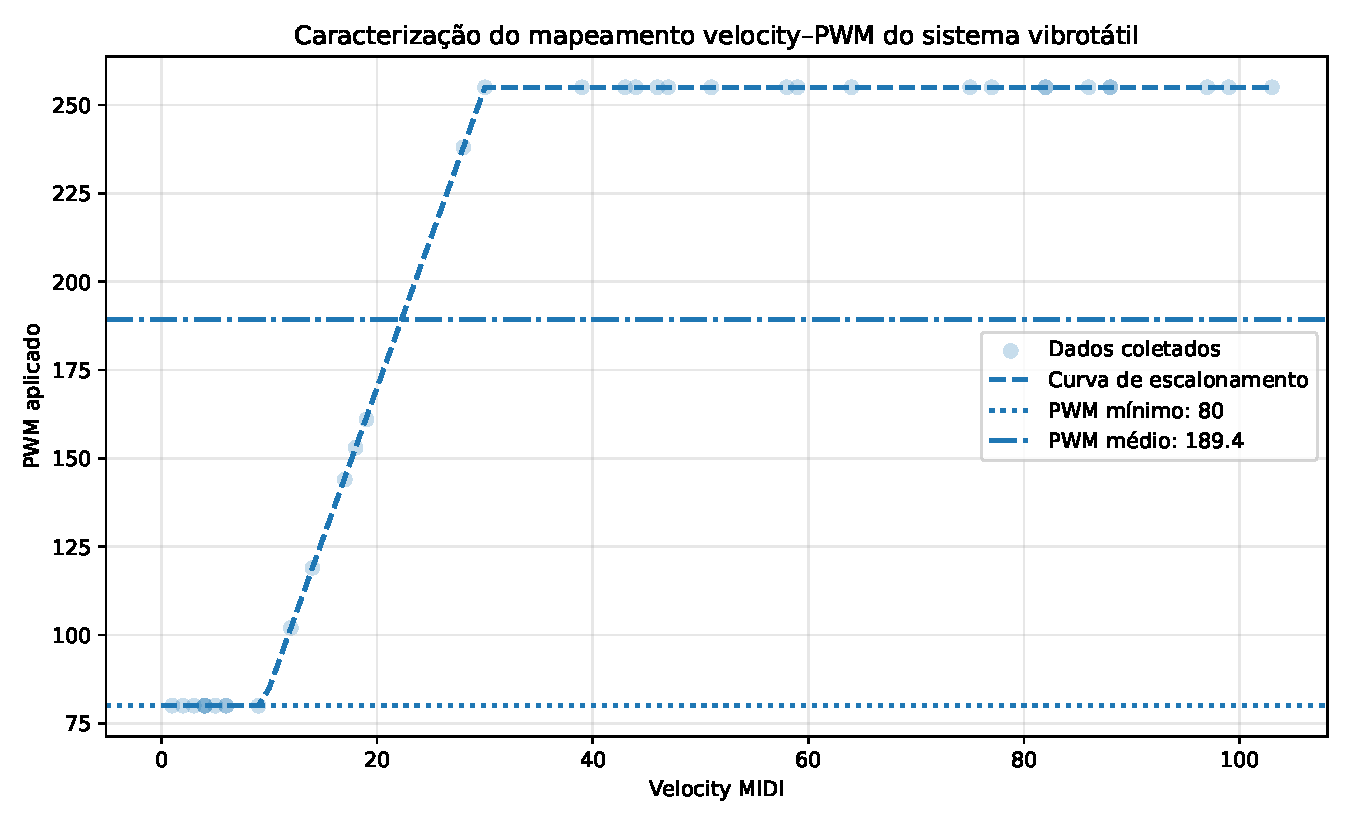
\includegraphics[width=0.85\linewidth,keepaspectratio]{Metodologia/grafico_velocity_pwm_final.pdf}
\caption{Relação experimental entre \textit{velocity} MIDI e valor PWM calculado}
\label{fig:curva_velocity_pwm}
\legend{Fonte: Elaboração própria (2026).}
\end{figure}

Os registros confirmaram o comportamento previsto pelo algoritmo: os comandos permaneceram entre 80 e 255, com limite inferior para acionamentos válidos, crescimento proporcional na região intermediária e saturação no valor máximo. A média dos valores PWM registrada no conjunto representado foi de 189,4. Essa relação é digital e não permite inferir uma proporcionalidade entre o comando e a intensidade mecânica ou luminosa percebida.

Nos ensaios posteriores com estímulo mecânico controlado, o MPD218 produziu frequentemente valores de \textit{velocity} superiores a 30, referência utilizada no programa principal. Para evitar a saturação precoce na caracterização experimental da Seção~\ref{sec:resultado_queda_controlada}, foi empregado um programa distinto que distribui a faixa MIDI de 1 a 127 entre PWM 80 e 255. As duas estratégias estão documentadas nos arquivos complementares do projeto.

\section{Resultados da Comunicação UDP}
\markright{Resultados e Discussão}
\label{sec:resultados_udp}


O procedimento de avaliação da comunicação UDP descrito na Seção~\ref{sec:teste_estabilidade_udp} foi utilizado para verificar o comportamento da transmissão sucessiva de comandos entre o software desenvolvido em Python e o microcontrolador ESP32.

O ensaio foi realizado com o envio de 100 pacotes numerados sequencialmente, com intervalo aproximado de 50~ms entre transmissões consecutivas, após a mensagem preliminar de inicialização definida na metodologia.

A análise considerou tanto a correspondência entre os identificadores transmitidos e recebidos quanto o comportamento temporal observado durante a sequência experimental.

\subsection{Recepção dos Pacotes}
\markright{Resultados e Discussão}
\label{sec:resultado_recepcao_udp}

A comparação entre os registros de transmissão e recepção mostrou que os 100 pacotes considerados no ensaio foram registrados pelo ESP32.

A figura a seguir apresenta os registros obtidos nos terminais utilizados durante o experimento.

\begin{figure}[!htbp]
\centering
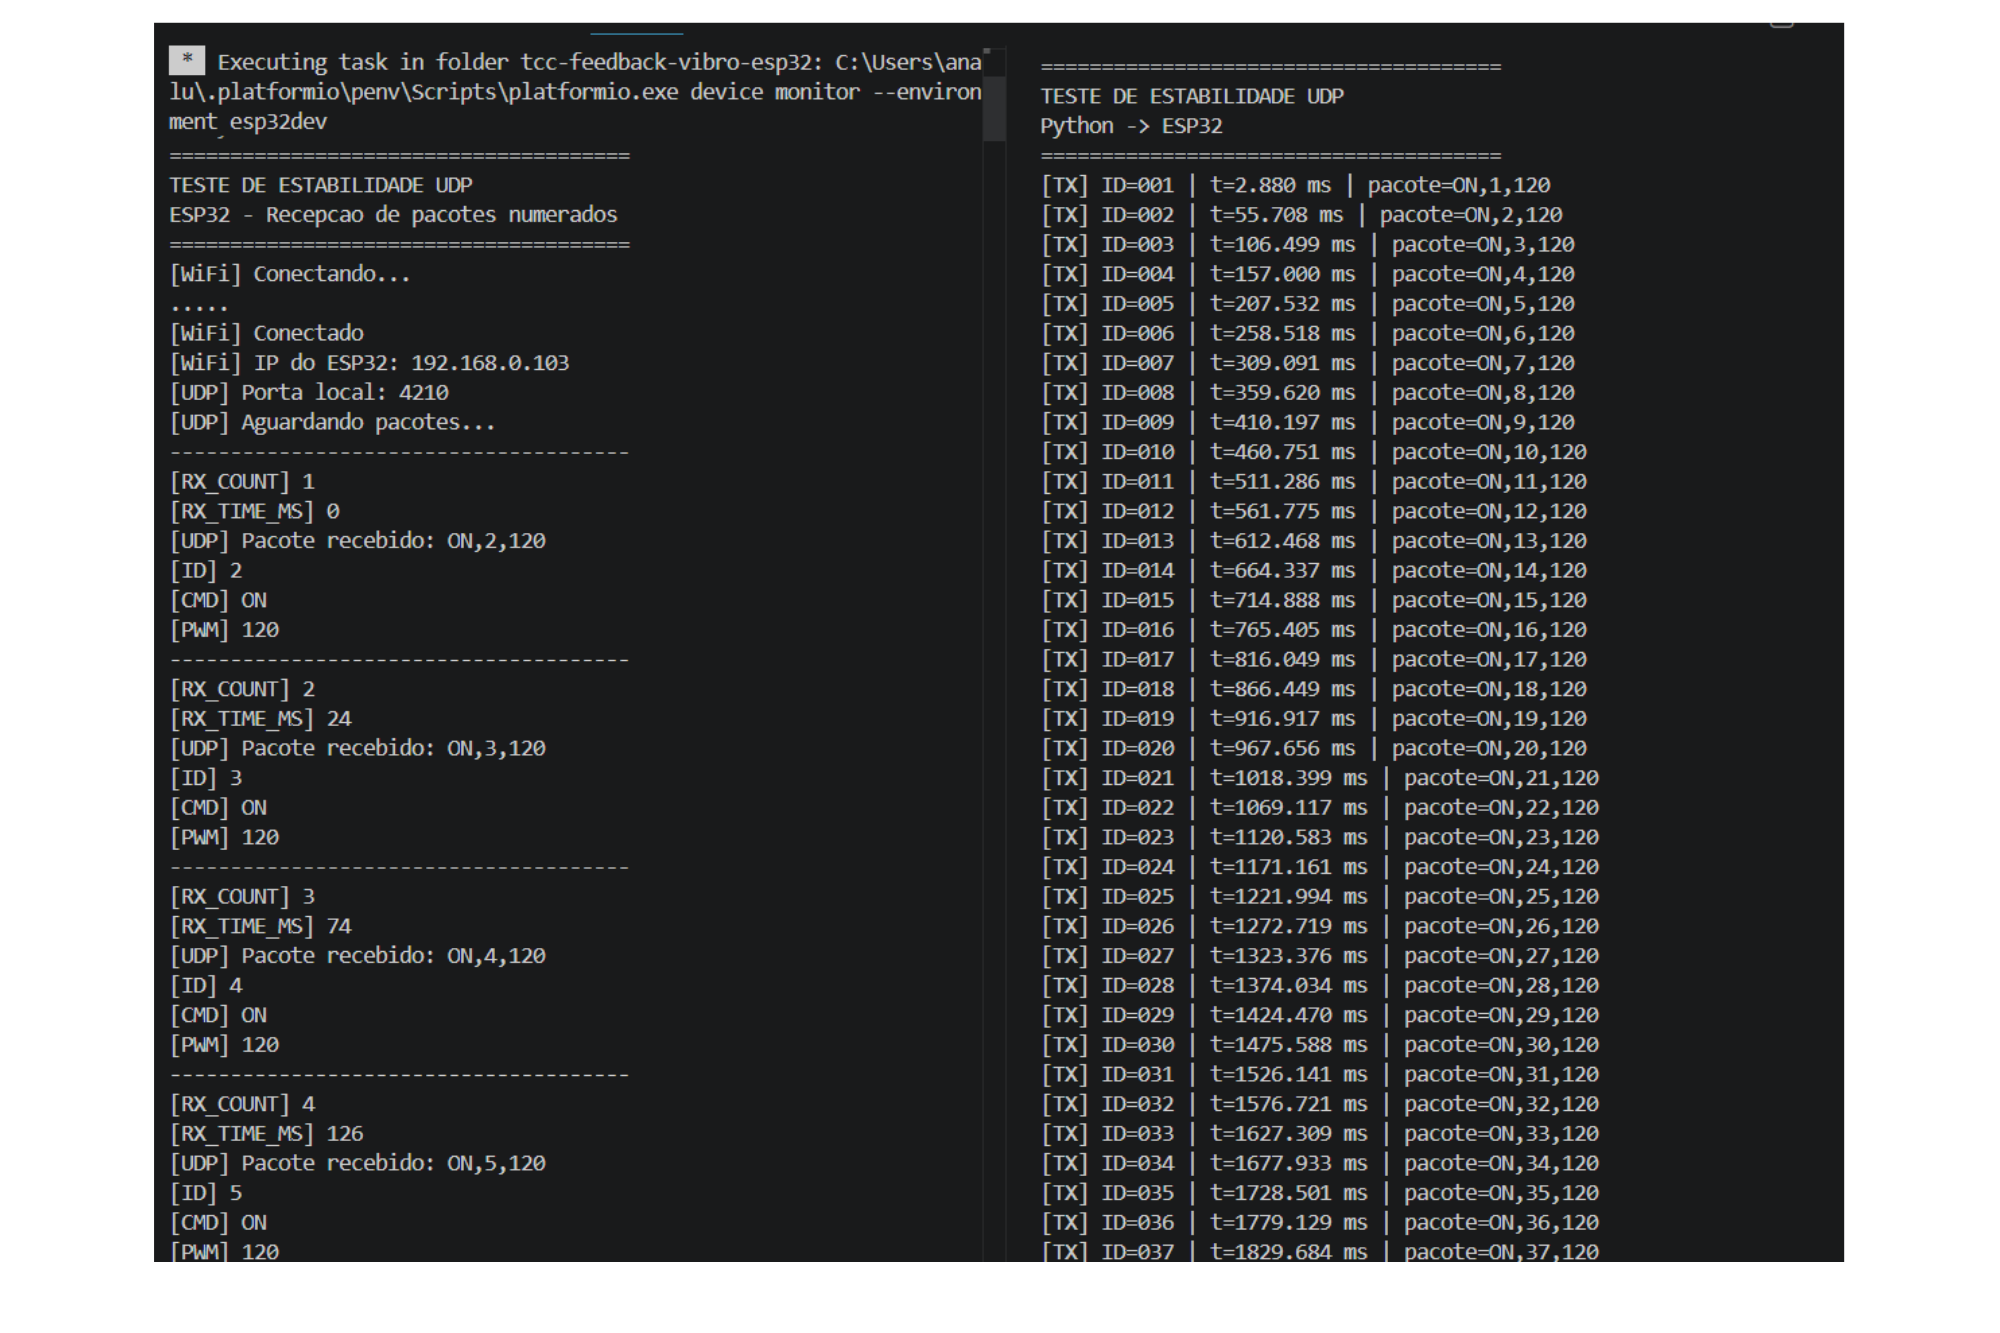
\includegraphics[
width=0.98\linewidth,
keepaspectratio
]{Metodologia/teste_estabilidade_terminal.png}
\caption{Registros do teste de transmissão de pacotes UDP entre Python e ESP32}
\label{fig:teste_estabilidade_udp_terminal}
\legend{Fonte: Elaboração própria (2026).}
\end{figure}

No terminal do software desenvolvido em Python foram registrados os identificadores dos pacotes transmitidos, enquanto o monitor serial do ESP32 permitiu acompanhar os identificadores efetivamente recebidos pelo microcontrolador.

Para a sequência analisada, foi observada correspondência entre os identificadores enviados e recebidos.

Os 100 datagramas considerados no ensaio foram registrados pelo ESP32, não sendo observada perda de pacotes na sequência utilizada para essa avaliação.

Esse resultado atende ao critério de validação estabelecido para a comunicação nas condições experimentais adotadas.

Entretanto, esse resultado deve ser interpretado dentro das condições específicas do ensaio. O protocolo UDP não incorpora mecanismos próprios de confirmação de entrega ou retransmissão e a ausência de perdas nessa sequência não constitui garantia de entrega dos datagramas em outras condições de rede, períodos mais prolongados de operação ou ambientes com diferentes níveis de interferência.

\subsection{Comportamento Temporal da Comunicação}
\markright{Resultados e Discussão}
\label{sec:resultado_temporal_udp}

Além da correspondência entre os pacotes transmitidos e recebidos, foram analisados os registros temporais produzidos durante o ensaio.

A figura a seguir apresenta o comportamento temporal da sequência de pacotes registrada pelo ESP32.

\begin{figure}[!htbp]
\centering
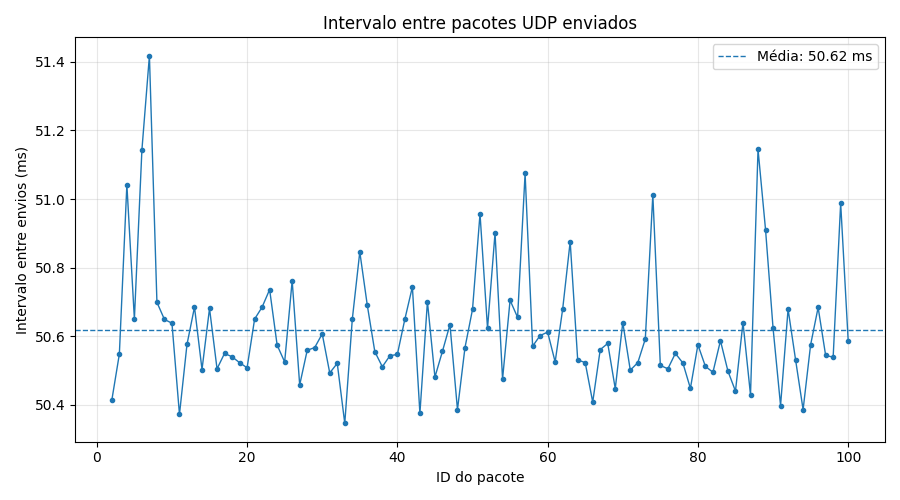
\includegraphics[
width=0.90\linewidth,
keepaspectratio
]{Metodologia/grafico_estabilidade_udp.png}
\caption{Comportamento temporal da recepção dos pacotes UDP durante o ensaio}
\label{fig:grafico_estabilidade_udp}
\legend{Fonte: Elaboração própria (2026).}
\end{figure}

Os registros apresentaram progressão temporal compatível com a transmissão sucessiva configurada no software, cujo intervalo nominal entre pacotes foi definido em aproximadamente 50~ms.

Foram observadas pequenas variações entre os intervalos de recepção ao longo da sequência.

Esse comportamento é compatível com a natureza não determinística da cadeia de comunicação utilizada, que envolve a execução do software no computador, a transmissão pela rede Wi-Fi, o processamento realizado pelo ESP32 e o próprio registro das informações pelo monitor serial.

Nas condições avaliadas, essas variações não impediram a recepção da sequência completa de pacotes considerada no ensaio.

O resultado permite caracterizar o funcionamento da comunicação UDP durante o procedimento realizado, mas não corresponde a uma medição da latência fim a fim do sistema.

Os instantes utilizados no computador e no ESP32 foram obtidos em plataformas distintas e sem uma referência temporal comum de alta precisão. Dessa forma, esses registros não foram utilizados para determinar quantitativamente o tempo transcorrido entre o acionamento de um pad MIDI e o início da resposta física do motor ou do LED.

Consequentemente, os resultados desta etapa sustentam a estabilidade funcional da transmissão nas condições experimentais adotadas, sem permitir classificar formalmente a arquitetura como um sistema de tempo real.

\section{Validação Física do Sistema Multissensorial}

A validação física do sistema foi realizada de forma incremental, conforme os procedimentos descritos no Capítulo 4.

A sequência de ensaios compreendeu inicialmente a verificação do estágio eletrônico utilizando uma carga auxiliar de teste, seguida pela validação do canal vibrotátil, integração da alimentação embarcada, incorporação do feedback visual e, por fim, operação simultânea das modalidades tátil e visual com a unidade vestível alimentada pelas baterias.

Essa abordagem permitiu verificar individualmente os principais módulos físicos antes da operação integrada da arquitetura.


\subsection{Validação do Estágio de Chaveamento}
\markright{Resultados e Discussão}

Na etapa inicial de validação física, um LED foi utilizado como carga auxiliar de teste no estágio de chaveamento baseado no transistor MOSFET IRLZ44N.

A aplicação dos comandos de controle permitiu verificar o caminho formado pelo GPIO do ESP32, resistor de gate, transistor MOSFET e carga conectada à saída.

A resposta observada confirmou a capacidade do ESP32 de comandar o estágio eletrônico antes da conexão do motor vibrotátil.

Esse procedimento reduziu o risco associado à integração inicial com a carga indutiva e permitiu prosseguir para a utilização do atuador Vibracall 1027.

O LED empregado nessa etapa teve função exclusivamente auxiliar de depuração e não corresponde ao canal de feedback visual posteriormente incorporado à configuração final do protótipo.


\subsection{Validação do Canal Vibrotátil}
\markright{Resultados e Discussão}

Após a validação inicial do estágio de chaveamento, foi realizado o ensaio utilizando um motor Vibracall 1027 conectado ao circuito eletrônico.

Durante a primeira etapa de depuração, foram realizadas medições de tensão e testes de continuidade entre o GPIO 18 do ESP32, o resistor de gate e o terminal de controle do MOSFET.

Foi identificada uma falha de contato no caminho entre a saída do microcontrolador e o estágio de gate, impedindo que o nível lógico produzido pelo ESP32 chegasse adequadamente ao transistor.

Após a correção da conexão, foi verificada a presença de aproximadamente 3,3~V no estágio de controle durante a condição de acionamento.

Em seguida, comandos UDP foram enviados diretamente ao ESP32 para verificar o acionamento e o desligamento do motor.

O Vibracall 1027 passou a responder corretamente aos comandos recebidos, confirmando o funcionamento da cadeia formada pela comunicação UDP, geração do sinal PWM, estágio de chaveamento e atuador vibrotátil.

Posteriormente, o controlador Akai MPD218 foi utilizado como fonte dos eventos de entrada. O software desenvolvido em Python processou os valores de \textit{velocity}, calculou os respectivos comandos PWM e realizou sua transmissão ao ESP32.

Durante esse ensaio, o motor apresentou acionamento durante os eventos válidos e desligamento após o término da interação, confirmando o funcionamento do canal vibrotátil utilizando a cadeia completa de controle prevista na arquitetura.



\subsection{Resposta do MPD218 ao Ensaio com Corpo de Massa Conhecida}
\markright{Resultados e Discussão}
\label{sec:resultado_queda_controlada}

O ensaio com o corpo de 39~g permitiu avaliar a resposta do controlador sob condições de impacto progressivamente maiores. Foram realizadas dez repetições em cada uma das seis alturas definidas na metodologia, totalizando 60 quedas independentes. Em cada repetição foi considerado apenas o primeiro evento MIDI válido após o armamento do programa; os eventos subsequentes ocorridos dentro da janela temporal de filtragem foram registrados separadamente como repiques. O procedimento e o corpo utilizado são apresentados na Figura~\ref{fig:ensaio_queda_massa}, enquanto o ensaio exploratório que antecedeu a definição da metodologia é registrado na Figura~\ref{fig:ensaio_estatico_exploratorio}.

Nos ensaios exploratórios anteriores à coleta definitiva, foi registrada uma condição próxima de 579~g para a ocorrência de acionamento no carregamento estático do \textit{pad}, documentado na Figura~\ref{fig:ensaio_estatico_exploratorio}. Esse valor foi mantido como observação preliminar e não integrou a análise quantitativa principal. Alturas de queda superiores a 5~cm produziram ocorrência frequente do valor máximo de \textit{velocity}, igual a 127, além de impactos progressivamente mais severos sobre o controlador. Durante os ensaios preliminares observou-se que, após o primeiro contato com o \textit{pad}, o corpo podia retornar à superfície e produzir um ou mais eventos MIDI adicionais, motivando a filtragem de repiques descrita na Seção~\ref{sec:filtragem_repiques}.

A Tabela~\ref{tab:queda_velocity_pwm} resume os resultados obtidos. Além da média, são apresentados o desvio-padrão e a mediana da \textit{velocity}, de modo a evidenciar a dispersão observada principalmente nas menores alturas. Os valores de PWM correspondem ao mapeamento específico utilizado neste ensaio, com a faixa MIDI de 1 a 127 distribuída entre PWM 80 e 255.

\begin{table}[!htbp]
\centering
\caption{Resultados do ensaio com corpo de 39~g para diferentes alturas de queda}
\label{tab:queda_velocity_pwm}
\resizebox{\textwidth}{!}{
\begin{tabular}{c c c c c c c}
\hline
Altura (cm) & $E_p$ (J) & \textit{Velocity} média $\pm$ DP & Mediana & PWM médio $\pm$ DP & Repiques & $v=127$ \\
\hline
0,5 & 0,001912 & 38,6 $\pm$ 19,91 & 41,0 & 132,2 $\pm$ 27,61 & 0 & 0 \\
1,0 & 0,003825 & 76,9 $\pm$ 26,49 & 87,0 & 185,5 $\pm$ 36,70 & 4 & 0 \\
2,0 & 0,007649 & 99,4 $\pm$ 9,29 & 102,0 & 216,6 $\pm$ 12,93 & 8 & 0 \\
3,0 & 0,011474 & 108,5 $\pm$ 5,56 & 111,0 & 229,3 $\pm$ 7,90 & 7 & 0 \\
4,0 & 0,015298 & 116,3 $\pm$ 7,72 & 118,5 & 240,0 $\pm$ 10,61 & 4 & 0 \\
5,0 & 0,019123 & 124,5 $\pm$ 2,01 & 124,5 & 251,4 $\pm$ 2,88 & 3 & 3 \\
\hline
\end{tabular}
}
\legend{Fonte: Elaboração própria (2026).}
\end{table}

Observa-se crescimento sucessivo da média de \textit{velocity} ao longo de todas as condições avaliadas. O valor médio passou de 38,6 na altura de 0,5~cm para 124,5 em 5~cm. Como o PWM foi calculado a partir da \textit{velocity}, a mesma tendência foi preservada na variável de controle, cuja média aumentou de 132,2 para 251,4.

A dispersão foi mais elevada nas duas menores alturas. Para 0,5~cm e 1~cm, os desvios-padrão de \textit{velocity} foram, respectivamente, 19,91 e 26,49. A partir de 2~cm, a variabilidade diminuiu de forma acentuada, com desvios entre 2,01 e 9,29. As observações válidas das menores alturas foram mantidas na análise, inclusive quando apresentaram valores reduzidos, pois correspondiam ao primeiro impacto registrado após o armamento da repetição e não atendiam ao critério definido para classificação como repique.

Na condição de 5~cm, três das dez repetições atingiram o limite superior do protocolo MIDI, com \textit{velocity} igual a 127. Esse comportamento indica o início de uma região de saturação do próprio controlador para as condições adotadas. A escolha de alturas mais elevadas tenderia a reduzir a capacidade do ensaio de distinguir novos aumentos na intensidade do impacto.

A associação entre altura de queda e \textit{velocity} foi avaliada a partir das 60 observações individuais. O coeficiente de Spearman foi $\rho=0{,}944$ ($p<0{,}001$), indicando associação monotônica forte entre o aumento da altura e a resposta fornecida pelo MPD218. Como medida complementar, o coeficiente de Pearson foi $r=0{,}818$ ($p<0{,}001$). A diferença entre os dois coeficientes é compatível com a forma não estritamente linear da resposta e com a aproximação do limite superior de \textit{velocity} nas maiores alturas.

Esses resultados não representam uma medição direta da força de impacto. Para massa constante, o aumento da altura elevou a energia potencial disponível antes da queda e a velocidade teórica imediatamente anterior ao contato. O ensaio mostra que condições mecânicas de entrada progressivamente maiores produziram, em média, valores também maiores de \textit{velocity}, que foram convertidos em níveis crescentes de PWM pelo programa de teste.

A Figura~\ref{fig:altura_velocity_ensaio} apresenta a evolução da média de \textit{velocity} em função da altura de queda. As barras verticais correspondem a um desvio-padrão em torno da média de cada condição.

\begin{figure}[!htbp]
\centering
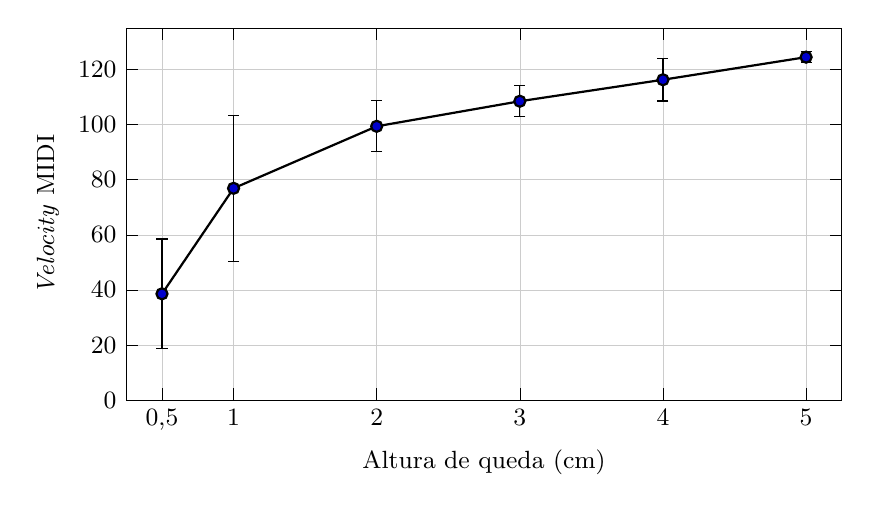
\begin{tikzpicture}
\begin{axis}[
    width=0.88\textwidth,
    height=0.52\textwidth,
    xlabel={Altura de queda (cm)},
    ylabel={\textit{Velocity} MIDI},
    xmin=0.25,
    xmax=5.25,
    ymin=0,
    ymax=135,
    xtick={0.5,1,2,3,4,5},
    xticklabels={{0,5},1,2,3,4,5},
    ytick={0,20,40,60,80,100,120},
    grid=major,
    major grid style={line width=.2pt,draw=gray!40},
    axis line style={black},
    tick style={black},
    tick label style={font=\small},
    label style={font=\small},
    legend style={font=\small,draw=none,at={(0.03,0.97)},anchor=north west},
]
\addplot+[
    color=black,
    mark=*,
    thick,
    error bars/.cd,
    y dir=both,
    y explicit
] coordinates {
    (0.5,38.6) +- (0,19.91)
    (1,76.9)   +- (0,26.49)
    (2,99.4)   +- (0,9.29)
    (3,108.5)  +- (0,5.56)
    (4,116.3)  +- (0,7.72)
    (5,124.5)  +- (0,2.01)
};
\end{axis}
\end{tikzpicture}
\caption{Valor médio de \textit{velocity} em função da altura de queda do corpo de 39~g. As barras representam $\pm 1$ desvio-padrão.}
\label{fig:altura_velocity_ensaio}
\legend{Fonte: Elaboração própria (2026).}
\end{figure}




\subsection{Caracterização Acústica do Atuador em Função do PWM}
\markright{Resultados e Discussão}
\label{sec:resultado_acustico_pwm}

A caracterização acústica foi utilizada como uma segunda forma de observar o comportamento do motor diante de diferentes níveis de comando. Para cada valor de PWM foram analisadas três repetições, obtidas a partir da sequência automatizada de acionamento descrita na Seção~\ref{sec:ensaio_acustico_pwm}. A montagem utilizada para a captação é apresentada na Figura~\ref{fig:ensaio_microfone_condensador}.

A Tabela~\ref{tab:frequencia_pwm} apresenta as frequências acústicas identificadas em cada repetição, além da média, do desvio-padrão e do coeficiente de variação de cada condição.

\begin{table}[!htbp]
\centering
\caption{Frequência acústica associada ao funcionamento do motor para diferentes valores PWM}
\label{tab:frequencia_pwm}
\resizebox{\textwidth}{!}{
\begin{tabular}{c c c c c c c}
\hline
PWM & Rep. 1 (Hz) & Rep. 2 (Hz) & Rep. 3 (Hz) & Média (Hz) & DP (Hz) & CV (\%) \\
\hline
80  & 91,5  & 92,9  & 90,2  & 91,5  & 1,35  & 1,5 \\
115 & 106,3 & 127,9 & 126,5 & 120,2 & 12,09 & 10,1 \\
150 & 145,3 & 154,8 & 165,5 & 155,2 & 10,11 & 6,5 \\
185 & 173,6 & 191,1 & 196,5 & 187,1 & 11,97 & 6,4 \\
220 & 203,2 & 212,6 & 216,7 & 210,8 & 6,92  & 3,3 \\
255 & 224,8 & 227,4 & 231,5 & 227,9 & 3,38  & 1,5 \\
\hline
\end{tabular}
}
\legend{Fonte: Elaboração própria (2026).}
\end{table}

A frequência média aumentou em todas as etapas do ensaio, passando de aproximadamente 91,5~Hz para PWM 80 a 227,9~Hz para PWM 255. Considerando as 18 observações individuais, foi obtido coeficiente de Spearman $\rho=0{,}988$ ($p<0{,}001$) e coeficiente de Pearson $r=0{,}984$ ($p<0{,}001$). Os dois resultados indicam associação forte entre o nível de PWM aplicado e a frequência acústica identificada na gravação.

Como não havia um valor de referência nominal de frequência para cada nível de PWM nas condições específicas de montagem do protótipo, não foi calculado erro absoluto em relação a um valor verdadeiro. A repetibilidade foi caracterizada pelo desvio-padrão e pelo coeficiente de variação entre as três repetições. A maior dispersão relativa ocorreu em PWM 115, com coeficiente de variação de 10,1\%, enquanto as condições de PWM 80 e 255 apresentaram coeficiente de variação próximo de 1,5\%.

Também foi observada, em parte das condições intermediárias, tendência de aumento da frequência nas repetições posteriores. Como a sequência de PWM foi aplicada sempre em ordem crescente, o ensaio não permite separar completamente o efeito do comando de possíveis efeitos associados ao tempo de funcionamento, aquecimento do motor, alimentação ou acoplamento mecânico durante a gravação. Essa variação foi preservada nos resultados e incorporada às medidas de dispersão.

A medida acústica deve ser interpretada como um indicador indireto do comportamento do atuador. O ensaio não determina a amplitude mecânica da vibração nem substitui uma caracterização realizada com acelerômetro. Ainda assim, a progressão observada acrescenta evidência experimental de que níveis distintos de PWM produzem estados dinâmicos distintos no motor.

Em conjunto com o ensaio de queda controlada, a caracterização estabelece experimentalmente a sequência entre uma entrada mecânica de maior intensidade, o aumento da \textit{velocity} MIDI, o aumento do comando PWM e a alteração da frequência acústica associada ao funcionamento do atuador.

A Figura~\ref{fig:pwm_frequencia_acustica} sintetiza a relação entre o comando PWM e a frequência acústica média identificada no atuador. As barras verticais representam um desvio-padrão calculado a partir das três repetições de cada condição.

\begin{figure}[!htbp]
\centering
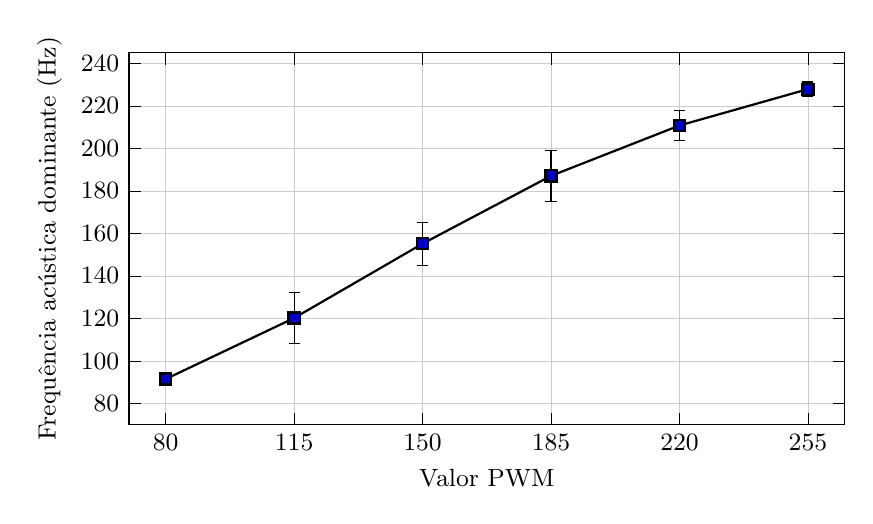
\begin{tikzpicture}
\begin{axis}[
    width=0.88\textwidth,
    height=0.52\textwidth,
    xlabel={Valor PWM},
    ylabel={Frequência acústica dominante (Hz)},
    xmin=70,
    xmax=265,
    ymin=70,
    ymax=245,
    xtick={80,115,150,185,220,255},
    ytick={80,100,120,140,160,180,200,220,240},
    grid=major,
    major grid style={line width=.2pt,draw=gray!40},
    axis line style={black},
    tick style={black},
    tick label style={font=\small},
    label style={font=\small},
]
\addplot+[
    color=black,
    mark=square*,
    thick,
    error bars/.cd,
    y dir=both,
    y explicit
] coordinates {
    (80,91.5)   +- (0,1.35)
    (115,120.2) +- (0,12.09)
    (150,155.2) +- (0,10.11)
    (185,187.1) +- (0,11.97)
    (220,210.8) +- (0,6.92)
    (255,227.9) +- (0,3.38)
};
\end{axis}
\end{tikzpicture}
\caption{Frequência acústica média associada ao funcionamento do motor em função do valor PWM aplicado. As barras representam $\pm 1$ desvio-padrão.}
\label{fig:pwm_frequencia_acustica}
\legend{Fonte: Elaboração própria (2026).}
\end{figure}




\subsection{Validação da Alimentação Embarcada}
\markright{Resultados e Discussão}

Após a validação do protótipo utilizando alimentação de bancada, foi realizada a integração do sistema destinado à operação autônoma da unidade vestível.

O conjunto de alimentação foi constituído por duas células recarregáveis de íons de lítio em configuração 2S, módulo BMS e conversor DC--DC baseado no MP1584EN. O módulo empregado nessa etapa é mostrado na Figura~\ref{fig:modulo_mp1584en}.

Antes da conexão ao circuito, a tensão de saída do conversor foi ajustada para aproximadamente 3,3~V.

Com o ESP32 em funcionamento e conectado à rede Wi-Fi, foram realizadas medições diretamente no barramento de alimentação do microcontrolador.

Durante os ensaios, foram observados valores aproximadamente entre 3,26~V e 3,29~V, indicando manutenção da alimentação próxima ao valor definido para operação do circuito.

Também foram realizados testes auxiliares de conectividade entre o computador e o ESP32 utilizando o comando \texttt{ping}. Após os ajustes realizados no estágio de alimentação e nas conexões físicas da montagem, o microcontrolador permaneceu conectado à rede utilizando exclusivamente a alimentação proveniente das baterias.

Esse resultado confirmou funcionalmente a possibilidade de operação da unidade vestível sem utilização da alimentação USB do computador.

A avaliação realizada concentrou-se na estabilidade funcional da alimentação durante os ensaios. Não foram realizados testes destinados à determinação da autonomia total das baterias, consumo médio de corrente ou eficiência energética do conjunto.


\subsection{Validação do Feedback Visual}
\markright{Resultados e Discussão}

O LED respondeu aos estados de acionamento e desligamento durante os testes com comandos enviados diretamente ao ESP32.

A aplicação de diferentes valores PWM também produziu alterações correspondentes no nível de acionamento luminoso observado durante os ensaios.

Esses resultados confirmaram o funcionamento do canal visual como uma saída física independente do canal vibrotátil, embora ambas as modalidades utilizem o mesmo valor digital de controle.

A validação realizada foi de caráter funcional. Não foram efetuadas medições fotométricas nem avaliação perceptiva da intensidade luminosa produzida pelo LED.


\subsection{Operação Integrada da Arquitetura}
\markright{Resultados e Discussão}

Na etapa final da validação física, foi avaliada a operação integrada da cadeia formada pelo controlador Akai MPD218, software desenvolvido em Python, interface gráfica, comunicação UDP sobre rede Wi-Fi, microcontrolador ESP32, motor Vibracall 1027, LED de alto brilho e sistema de alimentação embarcado.

Durante a interação com os pads, os eventos MIDI foram capturados pelo software, que identificou o valor de \textit{velocity}, calculou o valor PWM correspondente e transmitiu o comando ao microcontrolador.

O ESP32 aplicou o mesmo valor de controle ao GPIO 18, associado ao canal vibrotátil, e ao GPIO 21, associado ao canal visual.

Durante os ensaios, o acionamento de um pad resultou simultaneamente na vibração do motor e no acionamento do LED. Ao término do evento MIDI, o comando de desligamento interrompeu simultaneamente as duas modalidades de saída.

A interface gráfica executada no computador também respondeu aos eventos, apresentando as informações associadas ao pad acionado, ao valor de \textit{velocity} e ao valor PWM calculado.

A unidade embarcada permaneceu alimentada pelo conjunto de baterias durante essa etapa, sem necessidade de alimentação do ESP32 por meio da interface USB.

A configuração vestível obtida ao final da integração é registrada na Figura~\ref{fig:prototipo_final_vestivel}. A fotografia documenta a disposição física alcançada após a passagem da montagem de bancada para a placa, o invólucro impresso e a pulseira de fixação.

Dessa forma, foi verificado experimentalmente o funcionamento integrado da cadeia:

\begin{center}
\text{MPD218}
$\rightarrow$
\text{Python}
$\rightarrow$
\text{UDP/Wi-Fi}
$\rightarrow$
\text{ESP32}
$\rightarrow$
\text{PWM}
$\rightarrow$
\text{feedback vibrotátil + feedback visual}
\end{center}

O resultado demonstra a viabilidade funcional da arquitetura desenvolvida para transformar informações provenientes da interação musical em respostas sensoriais tátil e visual utilizando uma unidade vestível com alimentação própria.

Essa conclusão permanece restrita ao funcionamento técnico do protótipo. Os ensaios realizados não permitem estabelecer, por si só, benefícios perceptivos, de acessibilidade ou terapêuticos sem avaliações posteriores com usuários.


\section{Discussão Integrada dos Resultados}

A avaliação conjunta dos subsistemas permite examinar a continuidade da informação entre o gesto no controlador MIDI e as respostas físicas da unidade vestível. Os ensaios de entrada, processamento, comunicação e atuação foram realizados separadamente antes da integração, o que possibilitou identificar falhas de montagem e distinguir a resposta de cada etapa.

Na entrada, o ensaio de queda mostrou associação monotônica entre a altura de liberação do corpo e a \textit{velocity} registrada. Essa caracterização também evidenciou uma limitação do mapeamento inicialmente empregado no programa principal: a referência superior de \textit{velocity} igual a 30 leva à saturação antecipada do comando PWM. O mapeamento completo utilizado na caracterização experimental preservou uma faixa maior de valores de controle, sem modificar retrospectivamente a configuração do programa original.

Na saída vibrotátil, as simulações sustentaram a escolha do diodo de \textit{flyback} para a proteção do estágio de chaveamento e mostraram a influência da razão cíclica sobre a carga elétrica equivalente. O ensaio acústico, por sua vez, identificou frequências distintas para diferentes comandos PWM. Essas observações são complementares, mas não estabelecem uma relação quantitativa entre \textit{velocity}, amplitude mecânica aplicada à pele e intensidade percebida; para isso, seriam necessárias medidas mecânicas diretas e avaliações com participantes.

A comunicação UDP permitiu a operação da cadeia nas condições do ensaio, com registro de todos os 100 datagramas avaliados. Esse resultado caracteriza a transmissão observada, mas não mede a latência entre o gesto MIDI e a resposta física, nem assegura o mesmo desempenho sob outras condições de rede. Assim, o funcionamento integrado não deve ser confundido com uma validação temporal de sistema em tempo real.

A alimentação embarcada permitiu operar o ESP32 sem conexão USB com o computador, e o LED acrescentou uma saída física independente do estágio do motor. Ambas as modalidades responderam ao comando comum, mas não foi estabelecida equivalência perceptiva entre brilho e vibração. A contribuição do protótipo está, portanto, na integração tecnicamente funcional desses módulos e na disponibilidade de uma plataforma reproduzível para avaliações futuras de acessibilidade musical.

